
\documentclass[openany]{book}
\usepackage{graphicx} % images
\usepackage{wrapfig}
\usepackage{listings} % nice code layout
\usepackage[usenames]{color} % color
\definecolor{listinggray}{gray}{0.9}
\definecolor{graphgray}{gray}{0.7}
\definecolor{ans}{rgb}{1,0,0}
\definecolor{blue}{rgb}{0,0,1}
% \Verilog{title}{label}{file}
\newcommand{\Verilog}[3]{
  \lstset{language=Verilog}
  \lstset{backgroundcolor=\color{listinggray},rulecolor=\color{blue}}
  \lstset{linewidth=\textwidth}
  \lstset{commentstyle=\textit, stringstyle=\upshape,showspaces=false}
  \lstset{frame=tb, tabsize=2}
  \lstinputlisting[caption={#1},label={#2}]{#3}
}
\renewcommand{\chaptername}{Lab}
\newcommand{\WrapBarrier}{$\quad$\vspace*{-.225in}}


\title{ELC 3338 Project Book}
\author{Steve Potter}


\begin{document}

\maketitle
\tableofcontents


\chapter{Introduction}

n the Labs for this course we will be building a 64-bit computer, so we can understand how it works and how we can make a synthesizable machine in a hardware description language (HDL) like Verilog.  In this lab we will be building the counter that sequences all our computer's instructions.

A computer has to execute one instruction after another.  We will be building a system to count sequentially from some starting number.  Since this counter will be used to keep our program running in order, it is called the program counter.  Our system needs to hold its value, count, and be able to change the starting value.  We will break this into three components: a register (to hold the data), an incrementer (to count), and a mux (to select the count or a new starting value).  For today we will just build the register, simulate it, and show how to write up the lab.

\section{Program Counter}

The register is called the program counter, since it holds the actual count.  It is the heart of our system so it is where we will start.  We are going to make a module that explains how to build a register (a D flip-flop) in Verilog.  Consider the code in Listing~\ref{code:register}.  It is made up of three sections: a header (which has the include command), a port list or interface (which specifies the signals coming in or going out of our module), and a body or implementation (which describes how to build it).

\Verilog{Verilog code to make a register.}{code:register}{../code/1_fetch/register.v}

The first part is the header.  We will use this same header each time.  It tells the Verilog compiler to get all the data from a file called definitions.vh.  The extension vh is a Verilog header.  We use this to specify common pieces of data we will use across our design, so that all the components we build will be consistent.  By putting them in one file, we make it easier to maintain, and prevent mistakes that can happen easily by having multiple copies of these basic pieces of data.  For our first component the piece of data we will be using is WORD (set to 64), which is the size of the memory addresses our computer will use (how many bits).  Note that if we build things based around WORD, rather than the number 64, we can just change the value of WORD in the file and get a computer with a different size with a couple key strokes.

The second part is the port list or interface.  In this area we specify what signals are coming in (input), going out (output), or could go either direction (inout).  For outputs only, we could also have the output driven by a register (reg) or not (wire).  The other two types (input and inout) are only wires.  If you don't specify anything for any of the port types, you will get a wire - it is the default.  In our case we have four signals: three inputs, and one output that is a register.  The first two inputs are single wires.  One is the clock, which specifies the timing, and the other is reset, which clears the contents (makes the zero).  The final input is the value we want to store in memory, and I have called it D, following the convention of digital logic.  D has multiple bits that are numbered from WORD-1 down to 0.  Thus the leftmost bit is 63 in this case, and the rightmost bit is 0\footnote{If you want to be technical this is called little endian, since the little end (the least significant or unit bit) is going into the first memory location (bit 0).  If you reversed the order by putting the 0 first and the WORD-1 last it would be big endian, since the big end (most significant bit) would go in the lowest addressed bit.}.  If you changed WORD to be 64, this would automatically become 63 down to 0, which would resize the input.  Pretty cool\footnote{I grew up in the 80's so I reserve the right to say cool, rad, tubular, or any other 80's-ism.  :) }!  The output Q (also the digital logic conventional name) is a register (it will hold its value) and should also be of size WORD and follow the same order as the input D.

The final section is the body or implementation.  It is composed of a single thread of code, that will keep running (hence always).  It will run one time every time there is a positive edge (0 to 1 transition) for either the clock or reset.  Reset has higher priority, so if reset is asserted the register is cleared (Q is set to zero), otherwise the value of D is stored it Q.  That is it.  A nice, simple module.

\section{Testbench}

We now want to test this.  To test it, we need to tell the simulator to build a copy (instantiate) the module, and then we will need to supply the inputs and look at the outputs.  Consider the testbench in Listing~\ref{code:register_test}.

\Verilog{Verilog code to test a register.}{code:register_test}{../code/1_fetch/register_test.v}

Like our register it starts with our standard header, but this time there are no ports!  A testbench is providing all the signals to simulate the inputs to the unit under test (UUT) and thus does not need them.  This is how Verilog finds a top level simulation module - there are no ports.  In the body (implementation) we have a bunch of things.  First all the signals to our UUT must be declared.  Outputs always must go to wires (the outputs are driving them, and only wires can be driven).  Often inputs become registers since you will want to specify a value and have it continue till you give it a new value, though some can be wires if you had another unit that was supplying the values from its outputs.  In our case, the clock signal will be driven by a module names oscillator, which will give us a nice square wave with period CYCLE, which is another constant defined in our definitions.vh file.  The code thus makes an oscillator and a register, then runs the initial thread (it runs once at the start then never again)  The initial thread sets the value of the input then waits a CYCLE.  The last couple delays are not full cycles.  I did this for two reasons:
\begin{enumerate}
\item To show you how to make Verilog do calculations for you.
\item To remind you that the input won't necessarily be nice and perfectly timed to your register.  Unsynchronized signals happen, and is a frequent cause of problems, hence the need to test.
\end{enumerate}
This is by no means an exhaustive testbench, but run it and look at the output.  Does it do what you expect?  What else might you want to test?  Add this to your testbench and run it again to see if the register works.



\begin{figure}
\caption{Timing diagram.}\label{fig:registertiming}
\begin{center}
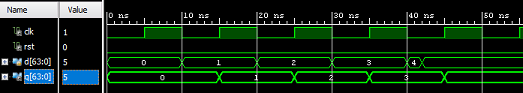
\includegraphics[width=4.75in]{../images/registertiming.png}
\end{center}
\end{figure}

\section{Using \LaTeX\ for Your Write-up}

All that is left is to write it up.  I am going to have you use \LaTeX\ to do your labs. Note how I include files, programs, and images.  It is worth noting that \LaTeX\ will automatically make the table of contents and bibliography for you also.  To top it off you only need a text editor as the files are just ASCII files.  To generate the document you run the command pdflatex and pass it the main file, and it will generate a pdf.

Why use \LaTeX\ ?  There are lots, but here are a few that matter in this course
\begin{enumerate}
\item It typesets programs from the actual source, no need to copy the program and have spell checkers and grammar editors mess things up.
\item It quickly and correctly handles equations (important given our math use).
\item It automatically handles table of contents and bibliographies.
\item It is free, and generates high quality documents (book quality) - it is open source since before open source.
\item It is used in publication of research documents.
\item It is the only large program believed to be error free in its source code, and have no missing features (development is complete!)
\end{enumerate}


\subsection{Background}

\TeX\ refers to both a language for typesetting and the program (compiler actually) that does the typesetting.  \LaTeX\ is a macro package which sits on top of \TeX\ and provides additional functionality, and has become synonymous with the language variant (dialect) of \TeX\ which it created.  Since \LaTeX\ is hugely popular and really useful, \TeX\ and \LaTeX\ have become synonymous to most people, and I will treat it so from now on.  A note on pronunciation: \TeX\ is in Greek letters - tau epsilon chi and hence is pronounced `tek' not tex (similar for \LaTeX\, which is pronounced `lay-tek' not latex).

\TeX\ is not a WYSIWYG (what you see is what you get) typesetting program like many editors you are familiar with, as it was designed to be a tagged language like the more recent html (yes, \TeX is older).  The idea is not to spend time thinking about how it should look, but rather to classify what it is and let the automated standards set the text by what the text is\footnote{For instance, note the chapter, section, and subsection commands in the tex files.  \LaTeX\ assigns a number, records it, the title, and page so it can automatically put it in the table of contents for you.}.  To provide flexibility and extension (and it was designed by one of the greatest computer scientists, Donald Knuth) it was set up as a programming language with a compiler.  You will thus interact with several different programs, an ASCII text editor (to write the files), a \TeX\ application to compile them, a pdf or dvi viewer to look at the output, and potential helper apps like dvi2ps, dvi2pdf, and their viewers.  Since \LaTeX\ is a programming language, we have a comment character \% that I had to escape by putting a \textbackslash before it to make it print.  Whitespace past the first space (word separation) is ignored, except for a blank line, which means start a new paragraph.  More than one blank line is ignored.  To get more space, you issue a command, such as \verb1\vspace{.25in}1, which puts a quarter inch of vertical space.  \LaTeX\ also knows pt (points), px (pixels), pc (pica), mm (millimeters), cm (centimeters), em (width of an `m'), and many more.  By default the space is not placed if it does not separate some object (i.e. at the top of a page), but you can force it by using \verb1\vspace*{.25in}1.  Starred commands are just versions of the main command.

There are many more commands than I can describe in this brief intro, including commands to let you define new commands and environments.  We will not need too many fancy commands, we only need to describe the commands to include figures, code, and equations.  If you want to learn more, then I have links to free manuals online at r2labs.org.

\subsection{Compile Process}

One thing that will help you a lot in working with \LaTeX\ is how the compile process works.  \TeX\ is a two pass compiler, but it does only one pass each time it runs.  Allow me a brief introduction to compilers, which is a great course if you can take it.

When you are compiling a file you have control statements (branches, loops, conditional execution statements like if or switch/case) that require you to know how many program lines ahead or behind something is in the assembled code, which you will not know at the start.   While you are often just putting in a flag or label to be handled by the assembler later, you in truth don't even know if they actually put the destination of the transfer of control, and thus have an error.  One easy way of handling this is to run through the process twice, collecting labels and such the first time and then doing the compile the second time through, which is what a two pass compiler does.  \TeX\ collects all the labels, notes all the chapter, section, and other structures, identifies all the bibliography references, and so on and puts them in a special auxiliary file for the next pass.  It will also create a DVI file, which has most things right, but will lack table of contents, references, bibliography, and such.  The second time through it already has the information before the file runs so it reads that first and uses it to create a fully correct output.

A logical question at this point is why not just have it run twice on its own?  Well, in the 1980's computers were small and slow, so each run of \TeX (we didn't even have \LaTeX\ at first) took an appreciable amount of time.  If you know the compile process, there are times you only have to run things once, like small spelling changes not in a title, chapter, etc.  Allowing people to do only one pass at a time was a big advantage (some \TeX\ compiles I had to do could take 10 minutes even in the 1990's).  Bibliographies are handled by an external program called BibTeX, which reads the .aux file to find the references (thus you need to run \LaTeX\ first), then pulls the data from the .bib files you specify in the calling command in your .tex file and creates a .bbl file.  The .bbl file contains all the info formatted how the bibliography should look.  \LaTeX\ reads this in the first pass and copies it over to the .aux file and resolves the links to the text references.  The next run of \LaTeX reads all this in and places both the bibliography and the cross references.  This means that to get a bibliography in you must run \LaTeX\, BibTeX, \LaTeX\, then \LaTeX\ once more.  You only need to do this if you add new reference, which in the labs will be once, provided you don't delete those intermediary files.

\section{Your Assignment}

You are to:
\begin{enumerate}
\item Finish the testbench in Listing~\ref{code:register_test}.
\item Run a simulation and generate a timing diagram like I did.
\item  Write up a lab report in \LaTeX\ following the lab format in \verb1LabN.tex1 and generate a pdf file.
\item Upload the pdf and all the Verilog files to the course LMS.
\end{enumerate} 

\chapter{Program Counter}

As mentioned in the last lab, the program counter is a register that is one word in length.  It holds the address in memory of the next instruction to be fetched and executed.  A typical program counter has to deal with a variety of situations that could change the program counter.  
\begin{enumerate}
\item The program counter should advance to the next address each cycle.
\item If the a branch is taken (from a conditional branch, unconditional branch, interrupt, or error), then the program counter should point to the branch's destination.
\end{enumerate}
The most typical is the computer must fetch instructions in sequential order.

\section{Incrementer}

We will build an incrementer by making a simple adder.  Later in our computer we will need another adder, so we will re-use this code.  When used as the program counter, we will pass it a 4 because each instruction is 32-bits long (even though it is a 64-bit computer) and we want to increment to the next instruction in memory.  Most machines are byte addressable, because one ASCII character (a char in c/c++) is a byte.  For a machine with 32-bit instructions like we are using, that would mean $32/8=4$ bytes to a word or each instruction would be 4 addresses later.  The book follows this convention so it will have 4 when it increments its program counter.

An adder is very simple in Verilog.  There are two inputs (the two numbers to be added) and one output (the result).   All the ports are size word because they hold integers.  

In this lab you will make your own adder and a testbench for the adder.  Your adder module should be called 'adder' and should have inputs of \verb1Ain1 and \verb1Bin1.  The output should be \verb1add_out1.

\section{Input Selection via Mux}

We will also need to be able to choose between normal advancing (sequential stepping) and branching (loops, if statements, etc.).  We will use a multiplexor (mux) to do this.  A mux is a simple device that connects one of the inputs to the outputs based on how the selector is set.  If the selector is 0 then input 0 is connected to the output, and if the selector is 1 then input 1 is connected to the output.  One interesting addition in this block of code is the addition of a size parameter.  Parameters are passed before the normal ports and are used to configure the code to meet a requirement at the time of construction.  Note parameters cannot change later.  The $=8$ defines the default value if nothing is specified.  In this case we are using parameters to set the number of wires that compose the inputs and output.  In our problem we will need some muxes to switch entire words (64 bits), but later we will also need to switch register addresses (5 bits).  Rather than write two muxes, we will make one and then use the parameter to change the size when they are declared.  The mux code is located in ARM-Lab/code/0\_common/mux.v.

\Verilog{Verilog code to make a mux.}{code:mux}{../code/0_common/mux.v}

Create a testbench for the mux.  Note that if the parameter is not set by the testbench, the mux module will set the inputs and outputs to be the default of 8.  We are going to change this to test it as a 64 bit mux.  In your testbench, instead of creating your mux module using \verb1mux UUT(...1, define the parameter as 64 by changing it to be \verb1mux#(64) UUT(...1  You can also do the dot notation as was done for the ports, but there are usually so few paramters you don't need to.  Now come up with good values to test your mux so you are confident it works.

\section{Your Assignment}

You are to:
\begin{enumerate}
\item Write an incrementer by creating an adder.	
\item Write a testbench for the adder.
\item Write a testbench for the mux in Listing.
\item Run a simulation and generate a timing diagram for each.
\item  Write up a lab report in \LaTeX\ following the lab format in \verb1LabN.tex1 and generate a pdf file.
\item Upload the pdf and all the Verilog files to the course LMS.
\end{enumerate} 
\chapter{Fetch Stage}

We are ready to build our fetch unit.  To do this, we will make one more unit, our instruction memory, then we will need to make a module to assemble all our units together.


\section{Instruction Memory}
The instructions are stored in memory, and are accessed by using the address where they are stored.  You can think of memory like a giant hotel for our data.  Each piece of data is stored in a room (memory location), which we can find by its room number (memory address).  To get a piece of data stored in memory (like an instruction) we need to take its address, go to that location, and grab the data.  A bunch of memory locations, accessed by an address is called an array.  Arrays in Verilog are declared like they are in C; the data type is specified, then the name, then the array size.  To store the instructions, we will need an array of 32-bit numbers (definitions.vh defines INSTR\_LEN as 32), which means the data type must be \verb2reg[`INSTR_LEN-1:0]2.  After the name is specified (mem in this case), we are going to use a parameter called SIZE to specify how big the array is: \verb2[SIZE-1:0]2.

The other interesting thing about this code is how to initialize the memory.  The default size of the memory is 1024 bytes, so we do not want to initialize this memory element by element in the code.  Fortunately Verilog gives you two functions to do this automatically: \$readmemb and \$readmemh.  The last letter specifies the base (binary or hexadecimal) of the data in the file.  White space separates fields, but the underscore character is ignored and thus can be used to make the values in a number more readable.  The readmemb function will be used to read the file `IMEMFILE and store the bits in the imem array.  This is done one time on initialization.  Then, you can access that data in imem at any time after that.  `IMEMFILE is defined in definitions.vh, and I provide this file, which contains 14 instructions.  However, you will need to update definitions.vh to point to your group's testfiles section rather than mine, or else it will not find the file.

\Verilog{Instruction Memory}{code:instmem}{../code/1_fetch/instr_mem.v}

The code is given in Listing~\ref{code:instmem}.  How will it be used?  What needs to be tested?  Consider those questions and write a testbench and verify it's operation.

\section{Fetch Stage}
Now we need to connect it together.  The components of our instruction fetch (sometimes called ifetch or just fetch) stage are shown in Figure~\ref{fig:fetch}.

\begin{wrapfigure}{L}{2in}
\caption{Instruction Fetch Stage.}\label{fig:fetch}
\begin{center}
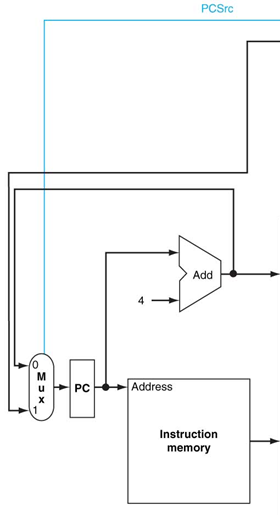
\includegraphics[width=2in]{../images/pipeline_fetch.png}
\end{center}
\end{wrapfigure}

Any wire (or reg) in the figure that comes in or goes out are input or output ports in the iFetch module.  In Figure~\ref{fig:fetch}, the blue wire is a control signal and comes ultimately from the control unit, which you will build in the decode stage.   Wires (or regs) that are completely contained in the figure are local to the iFetch module and are thus defined internally in the module.  The one exception to this is the current program counter (cur\_pc).  While there is no reason that it must be output from the iFetch module, I recommend making it an output so that it shows up on your simulation results, helping you to keep track of which instruction is currently executing.  

While the input and output signals are easily identified by the diagram, you must also determine the size of each signal and whether it is a wire or reg.  When you look at the figure I cut from a figure in the book, note that not every wire has a name.  If a wire is unlabeled, it is worth looking at other figures (like your text in chapter 4) to figure out what the signal is.  

IMPORTANT NOTE: Throughout your entire project, your signal names should follow the convention of the Freescale Semiconductor Verilog guide, which states that signal names should be all lower case, with words separated by an underscore.   

Once you have figured out all your connecting signals (wires and regs), you should identify the components you are going to use.  We have already created the modules, so now we just need to tell Verilog to instantiate them (build one) in the iFetch module.  Again choose your names wisely.  I have instantiated them for you in Listing~\ref{code:fetch}, but I haven't made the connections yet.  You must use knowledge gained from the wiring diagram to hook the components together with the available wires.  You should not need to create any more wires and registers.  It is just a matter of connecting the components together correctly.

The code, minus the connections, is listed below in Listing~\ref{code:fetch}.    

\Verilog{Starter code for the fetch stage.}{code:fetch}{../code/1_fetch/iFetch.v}

\section{Fetch Testbench}
Once you have made your connections, you should test the operation of the iFetch module by creating iFetch\_test.v.  You know you checked your individual modules, but there could be errors, or unexpected behavior when you put them together.  Sometimes weird timings between modules causes signals to be missed and such.  

Your testbench should set the inputs into the iFetch stage and verify that the correct outputs are produced. You should test both sequential operation (PC incrementing by 4) and branching.  When you test branching, keep in mind that my provided instruction file (instrData.data) only contains 14 instructions, so don't branch beyond the end of the file.

As we progress through this lab, you will learn how critical timing is.  Please look at the cur\_pc value and the instruction value and verify that the instruction that was fetched is the correct instruction, according to instrData.data and the current program counter.  Make sure to switch back and forth between sequential and branching to make sure that this works properly, 

\section{Your Assignment}
You are to:
\begin{enumerate}
\item Write a testbench for the memory in Listing~\ref{code:instmem}.
\item Finish the fetch stage and write a testbench to verify it.
\item Run the simulations and generate a timing diagrams.
\item  Write up a lab report in \LaTeX\ following the lab format in \verb1LabN.tex1 and generate a pdf file.
\item Upload the pdf and all the Verilog files to Canvas.
\end{enumerate} 
\chapter{Beginning to Decode}

\section{Instruction Decode}

The next stage in the datapath is the iDecode stage.  The iDecode stage evaluates the binary instructions (an output of the iFetch stage) and determines what needs to be done.  There are many aspects to the iDecode stage, and some get fairly complex.  But today we will begin the process of decoding that instruction by decomposing the instructions into the key parts of R-Type and D-Type instructions:
\begin{enumerate}
	\item Opcode
	\item Address (used only in D-Type instructions)
	\item Rm (used only in R-Type instructions)
	\item Rn
	\item Rd (though the book uses Rt for D-type instructions, we will use Rd for the last operand of D-type instructions)
\end{enumerate}   

To do this, you will create a new module called instr\_parse.  This module will simply read inputs and assign appropriate output values.  These outputs should be assigned on the clock edge with non-blocking procedural assignments.  While this might not seem important now, it will become important later.  The inputs should be a clk signal and a 32-bit instruction.  Outputs are listed for you above.  Although R-type and D-type instructions have different operands, you can treat them the same for now.  For instance, you can still assign an Address field on an R-type instruction, and you can still assign an Rm field on a D-type instruction.  In future labs, we will begin treating the instructions differently and ignore the unnecessary fields.  Notice how because of the commonality of instruction format, Opcode, Rn, and Rd are all universal across these instruction types.  Please remember to use the style specified in the previous lab, where all items are lower case with underscores separating them.  For instance, for Rd, you should use the signal name rd\_num.  Appending num on the end of the name indicates that this is the register number, not the value from the register.

To test this, you will need to create an instr\_parse\_test.v that will feed the module with a clock signal and instructions.  Then you can verify that your instructions are being parsed correctly.

\section{Register File}

Next, we will create the register file.  You will create a new module called regfile (in regfile.v).  The regfile module should retrieve data from the registers on the rising edge of read\_clk as well as write to the registers on the rising edge of write\_clk when the regWrite flag is set.  The regfile should use a verilog reg array.  You do not need to use the register module that you used for your program counter.  Since we don't currently have the ability to do loads and stores (since we don't have data memory yet), the values for the registers should be stored in a datafile, regData.data and read in during the initial block, just like we did with the instr\_mem.v file.  

Inputs to the module should include a signal called read\_clk and a signal called write\_clk as well as all inputs shown on the Register file in Figure~\ref{fig:register_file_cutout}.  The outputs should be the outputs of the Register file in Figure~\ref{fig:register_file_cutout}.  Use names such as read\_register1, read\_data2, etc.

You will need to write a testbench, regfile\_test.v, for this module as well.  It should provide values for each input and verify that the outputs match expected behavior.

\begin{figure}
	\caption{Expected Results}\label{fig:register_file_cutout}
	\begin{center}
		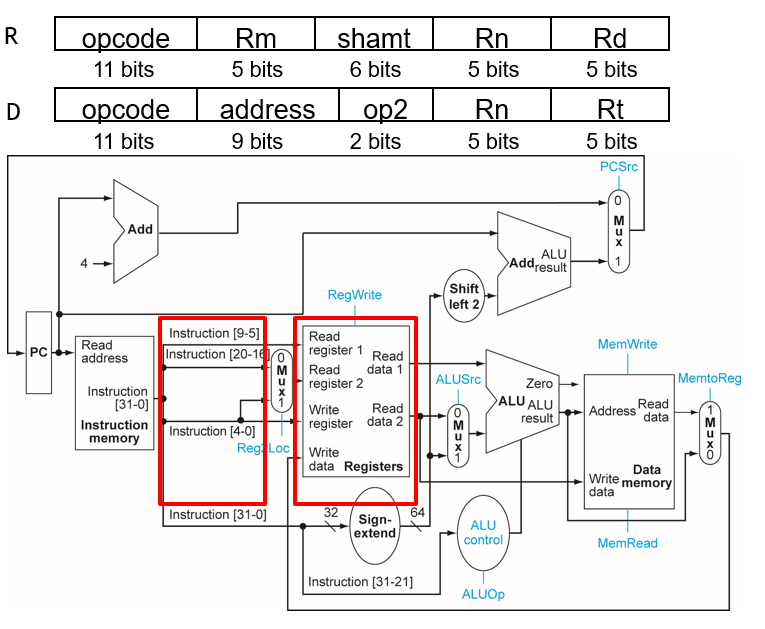
\includegraphics[width=4.75in]{../images/register_file_cutout.png}
	\end{center}
\end{figure} 


\clearpage
\section{Your Assignment}

You are to:
\begin{enumerate}
\item Create an instr\_parse module as described above.
\item Create an instr\_parse test module and verify that the instruction is being parsed properly.
\item Create a regfile module as described above.
\item Create a regfile\_test module and verify that the values are being stored and retrieved from the regfile properly.
\end{enumerate} 
\chapter{Register File}

\section{Register File}

Next, we will create the register file.  You will create a new module called regfile (in regfile.v), and this module will be part of your iDecode module.  The regfile module should retrieve data from the registers as well as write to the registers when the regWrite flag is set and the clock edge rises.  The regfile should use a verilog reg array.  You do not need to use the register module that you used for your program counter.  Since we don't currently have the ability to do loads and stores (since we don't have data memory yet), the values for the registers should be stored in a datafile, fibR.data and read in during the initial block.  In order to get results that match my provided results (and match the provided unit test), you should set X21=16, X9=33, X10=12 in fibR.data.

A unit test is provided, iDecode\_test.v.  It simply sends two commands (the add and subtract commands from last lab) and sets a few flags.  Using that unit test, you should be able to produce the results shown in the lab manual.  Note that in addition to the register file, you will also need to create a mux to determine the source of the second read register.  Note that because we are sending the instructions from the test instead of from the iFetch routine, you will need to update your code from last lab to use procedural statements triggered on the clock edge.  Otherwise, the instructions will not come in on the clock edge as expected.  Timing is very important in this lab.

\begin{figure}
	\caption{Expected Results}\label{fig:register_file_cutout}
	\begin{center}
		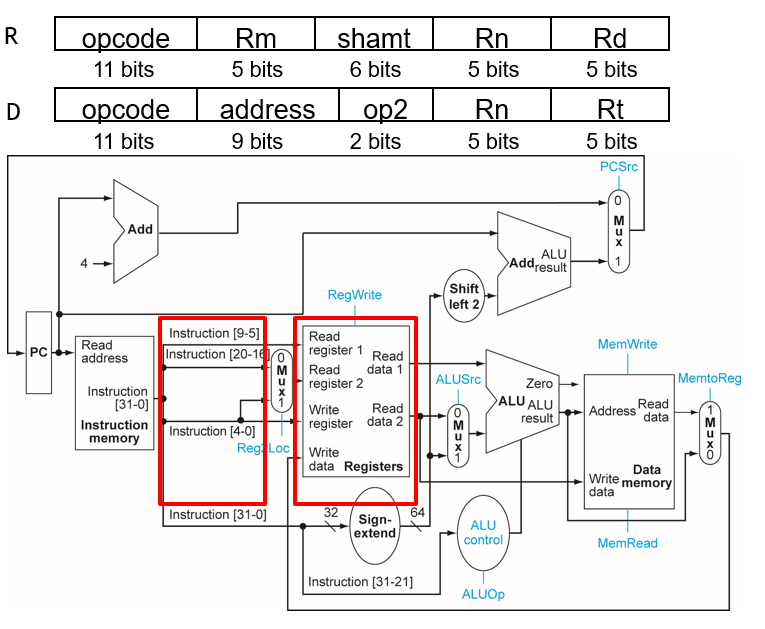
\includegraphics[width=4.75in]{../images/register_file_cutout.png}
	\end{center}
\end{figure} 

\Verilog{Verilog starter code for the iDecode module.}{code:iDecode_reg_test_version}{../code/2_decode/iDecode_reg_test_version.v}

\begin{figure}
	\caption{Expected Results}\label{fig:register_file_test_output}
	\begin{center}
		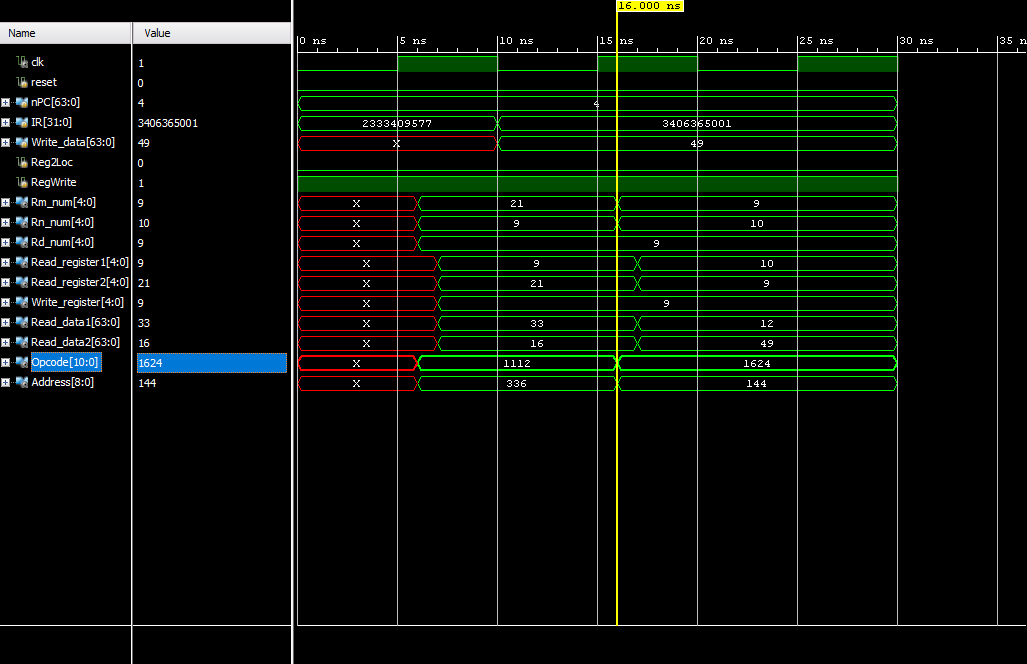
\includegraphics[width=6.75in]{../images/register_file_test_output.png}
	\end{center}
\end{figure}

\clearpage
\section{Your Assignment}

You are to:
\begin{enumerate}
\item Create a regfile module and add it to the iDecode module.
\item Re-use your mux from previous labs and add it to the iDecode module.
\item Import the provided iDecode\_test.v file.
\item Verify that your results match the expected results.
\item There will not be a submittal on Canvas today.  However, please show me your results either today or at the beginning of lab time during the next class period.  We will be adding more functionality next time.
\end{enumerate} 
\chapter{Finishing Decode}

\section{iDecode Module}
At this point, you have created all of the modules necessary to assemble the iDecode module.  Now you need to create a new module called iDecode.  The inputs and outputs can be determined by evaluating Figure~\ref{fig:decode_stage}.  Any signal that crosses the boundaries of the red box is an input or output.  Signals that do not cross the boundaries of the red box are signals that are internal to the iDecode module and should be declared internally in iDecode.  Please make sure to label signals consistently with lower case letters with words separated by underscores.  For example, read\_data1, write\_data, alu\_src.

\begin{figure}
	\caption{Expected Results}\label{fig:decode_stage}
	\begin{center}
		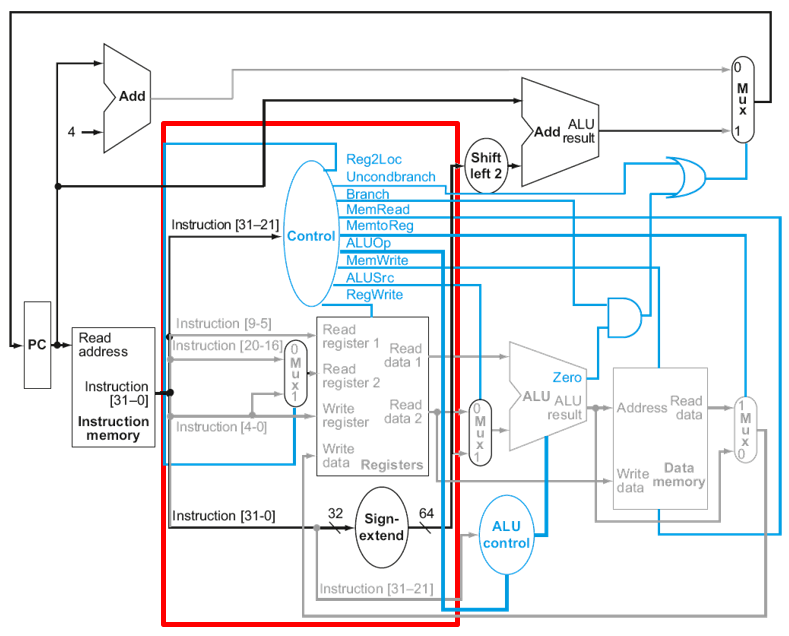
\includegraphics[width=4.75in]{../images/decode_stage.png}
	\end{center}
\end{figure} 


\section{iDecode Unit Test}
To verify that your iDecode module works correctly, you must first update your Expected Results Table. You should first add a row for every input and output of your iDecode module, then fill in all cells with expected values.  If a particular data item is not relevant for a particular instruction (for instance, sign\_extended\_output on an R-type instruction), then just put an X in that cell.  To ensure that we are testing each case, please update regData.data to reflect the following values:

\begin{enumerate}
	\item X19 = 10
	\item X20 = 30
	\item X21 = 0
	\item X22 = 16
\end{enumerate}

Now create a unit test for iDecode by providing the inputs for iDecode and verifying the outputs of iDecode.  For the instruction input, use the instructions from your Expected Results Table.  For arithmetic instructions, use the test bench to provide the correct value to the write\_data input, since we do not yet have an ALU to do the calculations.  Also, please use your test bench to provide a value of 20 to X9 in the first command (LDUR).

With your Expected Results Table in hand, you should be able to run the iDecode unit test and analyze your simulation outputs by going vertically down the simulation output, comparing the table to your simulation output.  While certain values will be offset in time, a single instruction should fall within a single clock cycle.  

\section{Integrating iFetch and iDecode}
Now that you have iDecode created and tested, you can test it with your iFetch module.  To do this, you need to create a file called datapath.v.  This will be your top-level file for your integrated datapath, analagous to the test bench files.  In this file, you should have an instance of iFetch and iDecode.  You should connect these two modules with wires by analyzing the full datapath diagram.  Since we do not have a full datapath yet, we need to have some "test bench" aspects to datapath.v.  Similarly to your iFetch test, you will want to create a reg for reset, pc\_src, and branch\_target.  Since we do not have all aspects of branching implemented, please keep pc\_src set to 0 for the duration of the test.  

Please update your instrData.data file to only contain the 10 instructions in your Expected Results Table.  The goal of datapath.v is to verify that the PC increments, each of these instructions is fetched at the appropriate time, and that the instruction executes properly.  You can verify the execution by comparing your results with your expected results table.     

\section{Your Assignment}

You are to:
\begin{enumerate}
\item Integrate all individual modules into the iDecode module.
\item Update your Expected Results Table to include all iDecode inputs and outputs.
\item Test the iDecode module with the instructions from the Expected Results Table.
\item Verify that your simulation results match your expected results.
\item Create datapath.v and integrate the iFetch and iDecode stages.
\item Verify that the results match the Expected Results Table.
\item Write a lab report according to the LabN format.  The focus of the report is the iDecode module, including testing it with iDecode\_test and integrating it with iFetch.  It does not need to describe the details of the submodules...you have already written a report on those.  Please consider datapath.v to be a testbench when writing the report.
\end{enumerate} 
\chapter{ALU and ALU Control}

\section{ALU}

First we will build the ALU itself.  The ALU has three inputs (two data inputs to act on, and a control input to determine the action perfomed) and two outputs (one data, and a logical flag). In the table shown in the lecture slides, you can see the meaning of the control bits used to determine what the ALU will calculate.  You should use a case statement for the control bits to determine which ALU operation to perform.  For each operation, you do not have to do anything fancy.  You just need to use the math capability that verilog provides to make the calculation.  You should give the the ALU control bits names in the definitions.vh file, and you should use these in your cases.  Also don't forget to make a default case, which is needed to actually wire this up.  Pick something fast for the default, thus usually a logic statement.

One last thing to note is the generation of the zero flag.  There are several ways to handle this, but the easiest way to handle it is below: 
\begin{enumerate}
\item In Verilog (like C), the statement $(a==b)$ is an operation with a boolean output.  You can thus say $x=(a==b);$ to assign $x$ to be the boolean value.  The statement $x=(a==b);$ is realizable as a digital comparator with $a$ and $b$ as inputs and $x$ as the single bit output.
\end{enumerate}

\section{ALU Control}

Now we need to build the controller to use the ALUOp field and the function field to generate the ALU control bits used above.  Consider the table for ALU Op to ALU Control bits in the lecture slides.  The ALU Control module is where you make this translation so that the ALU is told the proper operation to execute.  Use case statements and include a default to handle undefined signals (use fast commands for undefined signals).  Define the ALU operations in definitions.vh file to improve readability - you shouldn't need any numbers.  This should be a simple module with two inputs (ALUOp and function) and one output (control bits).

\section{Your Assignment}

You are to:
\begin{enumerate}
\item I have provided the test bench, ALU\_test.v.
\item Generate an ALU and ALU Control module and verify that you get the results that you expect.
\item Save your simulation results so that they can be included in a lab report.  We will not be submitting a lab report today.
\end{enumerate} 
\chapter{Execute Stage}

\section{Execute}

In the last lab, you created the ALU and ALU Control modules.  Now we will finish the iExecute stage.  The iExecute stage is represented by the red box in Figure ~\ref{fig:execute_stage}.  To finish the iExecute stage, you will need to add the following:
 
\begin{enumerate}
	\item Mux to select the source of the second input into the ALU.  You can reuse your mux that you created in the iFetch stage.
	\item Shifter to left shift the sign extended branch address offset.  You will need to create a new module for this.
	\item Adder to add the branch address offset to the current PC.  You can reuse your adder that you created in the iFetch stage.
\end{enumerate} 

\begin{figure}
	\caption{Execute Stage}\label{fig:execute_stage}
	\begin{center}
		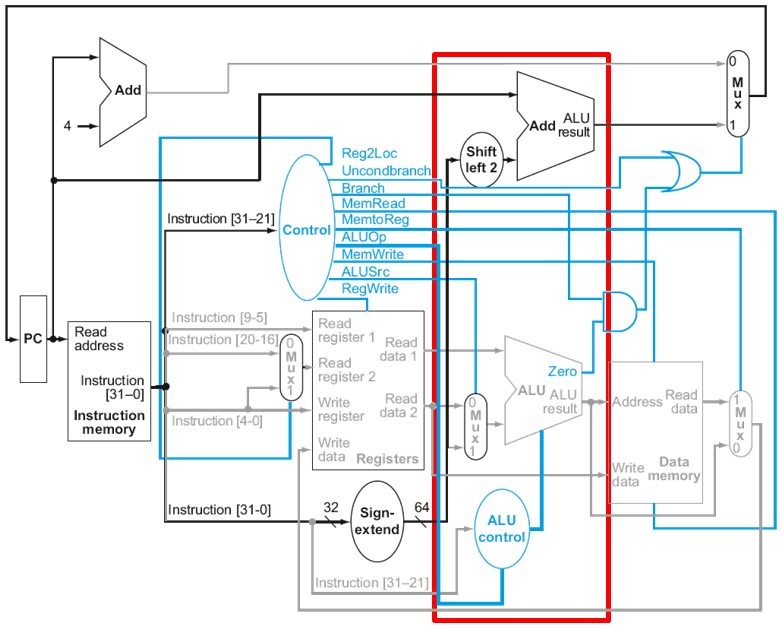
\includegraphics[width=4.75in]{../images/execute_stage.png}
	\end{center}
\end{figure} 

These five modules should be included in a new module called iExecute.  iExecute should consist of everything shown in the red box on Figure ~\ref{fig:execute_stage}. 

\section{Your Assignment}
I have provided a test bench, iExecute\_test.v.  Feel free to modify and improve it as you see fit.

You are to:
\begin{enumerate}
\item Complete the iExecute module and use the iExecute\_test to verify that you get the results that you expect.
\item Do not submit a lab report.  Move straight into Lab 9.
\end{enumerate} 
\chapter{Integrating Fetch and Decode}

\section{Integration}
We now have working Fetch, Decode, and Execute modules.  Now it is time to put them together to produce a system that can:
\begin{enumerate}
	\item Update the program counter
	\item Read the appropriate instruction from the instruction datafile
	\item Read the correct registers
	\item Update all control lines
	\item Sign extend address data
	\item Calculate Branch Target Addresses
	\item Provide a zero bit for conditional branch instructions
	\item Produce ALU results for R-Type and D-Type instructions
\end{enumerate}

Once we can do all of this, we will be ready for the iMemory stage.  We currently have the fetch and decode module integrated into datapath.v.  We also have a working execute module.  Today we need to integrate the Execute module into datapath.v.  You can reuse your instructions from fibI.data that you used when you integrated fetch and decode.  Please make sure that datapath.v is the "top module" in your project.  Once integrated, you should be able to produce a simulation that includes 3 new outputs:
\begin{enumerate}
	\item Branch Target
	\item ALU Result
	\item Zero
\end{enumerate}   

These three new outputs are marked on Figure Figure ~\ref{fig:integrated_execute}.  To verify these outputs, you should update the Expected Results Table that you made in Lab 7 to include these three outputs.  Then you should verify this table against your simulation results.

\begin{figure}
	\caption{Execute Stage}\label{fig:integrated_execute}
	\begin{center}
		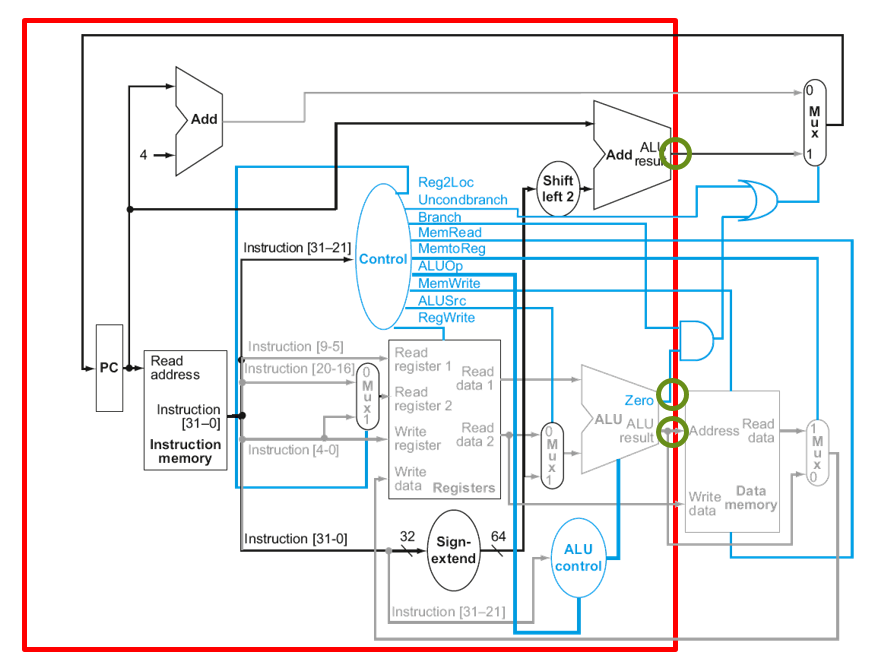
\includegraphics[width=4.75in]{../images/integrated_execute.png}
	\end{center}
\end{figure} 

\section{Your Assignment}

You are to:
\begin{enumerate}
\item Integrate your iExecute module into your datapath.v that includes iFetch and iExecute.
\item Update your Expected Results Table to include the new outputs.
\item Verify that your simulation results match your expected results.
\item This lab is relatively straightforward and does not warrant a full report.  Instead, make a short LaTex document (saved as PDF of course) with the following items:
\begin{enumerate}
	\item Expected Results Table
	\item Simulation Result Images
	\item datapath.v code
	\item A few sentences about the results, including anything that you don't believe is working correctly.
\end{enumerate}
\end{enumerate} 
\chapter{Memory}

\begin{center}
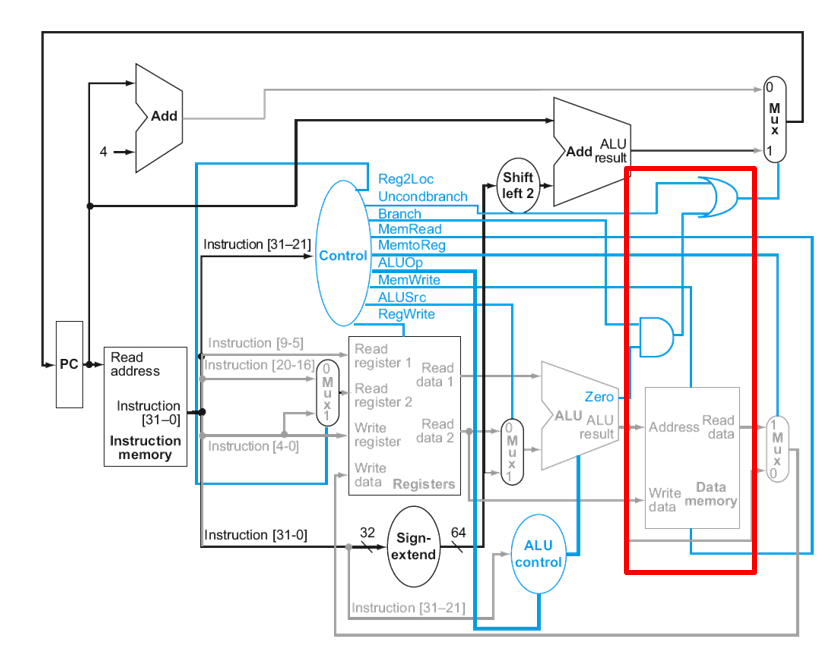
\includegraphics[width=5.5in]{../images/data_memory.png}
\end{center}


\section{Branch Resolution}

We now have all the information necessary to decide if the computer should branch or not.  We have the signal `branch' to tell us if it is a branch command, and we have `zero' to tell us if the condition was met.  Both branch and zero must be true so we will combine them with an `and' gate.

We also need an 'or' gate to 'or' together the output of the branch 'and' gate (above) and the uncondBranch control signal.  These gates can be included in your iMemory module as one line commands.  They do not need to be explicity tested, as they will be thoroughly tested when we integrate the system.  

\section{Data Memory}

This will be almost exactly like the instruction memory, with only two changes:
\begin{enumerate}
\item reading is now conditional on the `read' control wire being high.
\item writing is now permissible if the `write' control wire is high.
\end{enumerate}
As such, take your instruction memory (it is the right size, you could also use your register memory, but that would require more modification) and add the two changes above then test.

\section{Your Assignment}

You are to:
\begin{enumerate}
\item Create a new module called iMemory.
\item Instantiate the AND and OR gates directly in the iMemory stage.
\item Use instruction memory as a basis for a data memory module, and add the two new changes.  Also create or modify a fibD.data file.
\item Integrate data memory and the buffer into the iMemory stage.  
\item Write a testbench to verify that it works properly. Use a combination of fibD.data and testbench to test various scenarios.
\item There will not be a submittal for this lab.
\end{enumerate} 
\chapter{Write Back}


\begin{figure}
\caption{Write Back}\label{fig:wb}
\begin{center}
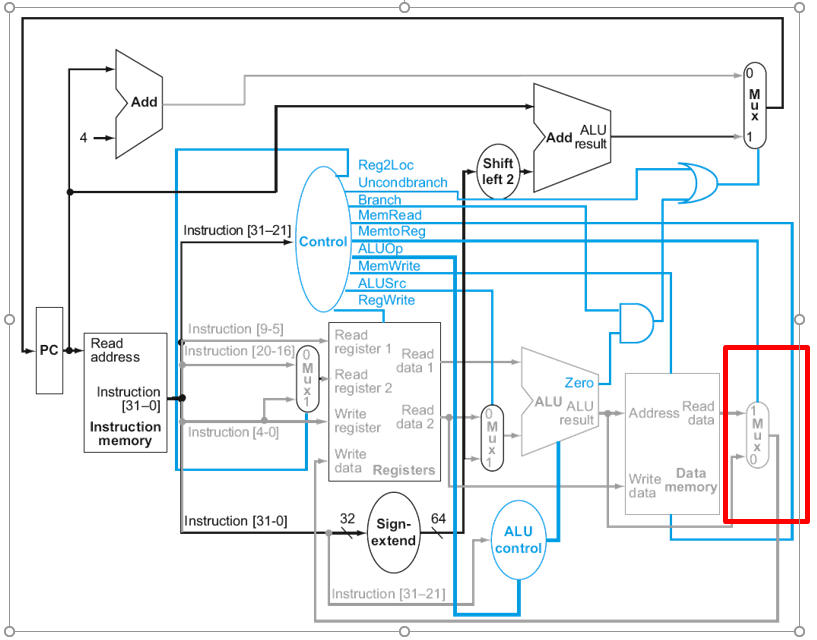
\includegraphics[width=\textwidth]{../images/writeback_stage.png}
\end{center}
\end{figure}

\WrapBarrier

\section{Mux}
This stage consists on only one item, a mux to select between the output of memory and the output of the ALU.  The control is the MemtoReg control line, see Fig~\ref{fig:wb}.  Since the mux has already been tested it does not need a testbench.  The stage thus has only 3 inputs (2 data and 1 control) and one output, the result.

\section{Datapath}
You are ready to assemble the full non-pipelined datapath shown in Fig~\ref{fig:datapath}.  To do this, you will need to combine all 5 stages into datapath.sv.  datapath.sv is the top-level file, so it is the testbench.  Verify operation of your datapath by running your set of instructions in instrData.data and testing the output.  These instructions are the 10 instructions from the Expected Results Table.  

Now that we have a writeback stage, we do not need to set write\_data in the initial section of datapath.sv.  Rather, you should connect write\_data from the WriteBack stage to the Decode stage.  Because we now have a memory stage, we should no longer need to set pc\_src in the inital section of datapath.sv.  However, our test instructions are not meant to run like a program and would yield strange results.  So for right now, we want to keep pc\_src hard-coded to 0 in datapath.sv.  To do this, we will use a new reg called pc\_src\_tmp and set it to 0.  Then we will use pc\_src\_tmp as the input to the iFetch module.  pc\_src will be a wire that is an output of the iMemory module.  In part 2 of this lab, we will get rid of pc\_src\_tmp and connect pc\_src from iMemory to iFetch.

I have provided a mostly complete datapath.sv.  The initial section is complete, including the cr values and all verifies.  Your job is to add your modules at the top and to define the clocks for those modules.  I have already added iFetch because I wanted to try to make it clear what we are doing with pc\_src\_tmp.  Once you add your modules and clocks, you should be able to run datapath.sv and get 175 test results (hopefully all passing!).

\begin{figure}
\caption{Full Non-Pipelined Datapath}\label{fig:datapath}
\begin{center}
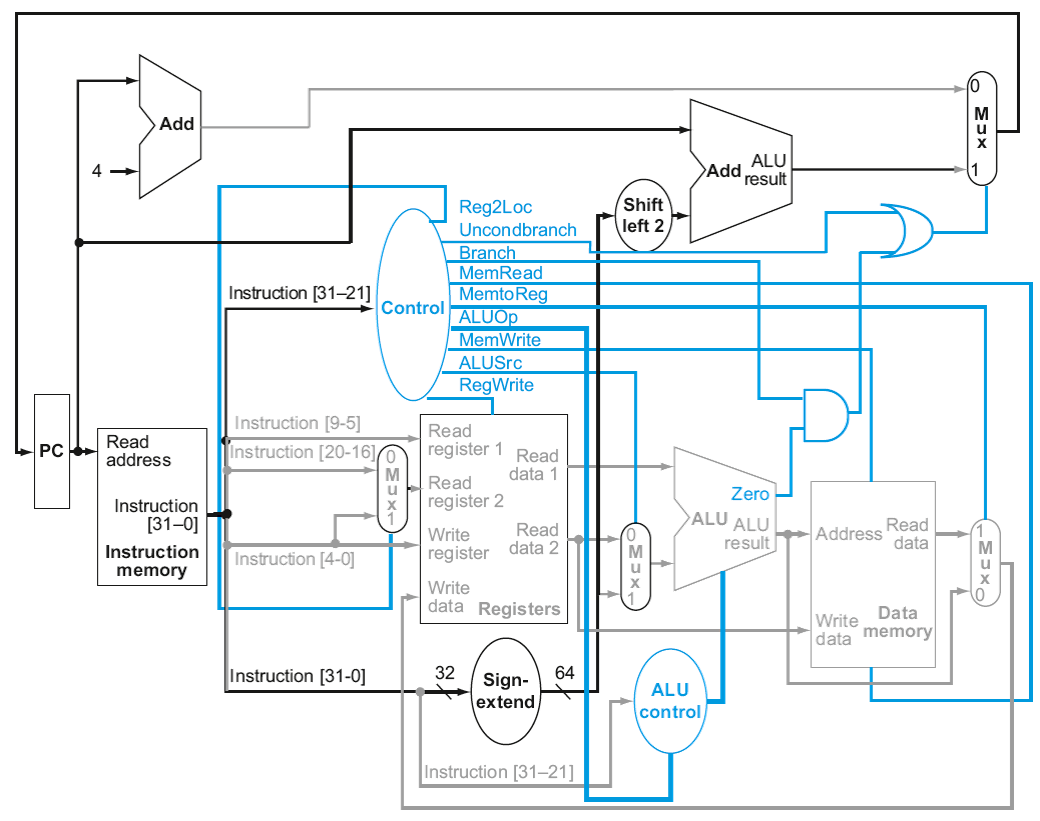
\includegraphics[width=\textwidth]{../images/non_pipelined_datapath.png}
\end{center}
\end{figure}

\section{Your Assignment Part 1}

You are to:
\begin{enumerate}
\item Update your Expected Results Table to include the iWriteBack stage.
\item Create the iWriteback stage consisting of one Mux.
\item Integrate all five stages into the file datapath.sv.
\item Run simulations to verify that your results match your Expected Results table.   
\item There will be one final test to add before we submit it.  However, please save copies of the following:
\begin{enumerate}
	\item A snip of the Simulation Results for datapath.sv.  Please show instructions in hex, opcodes and control signals in binary and everything else in signed decimal.  
	\item Copy and paste the entire log from BEGIN TEST RESULTS to END TEST RESULTS into your file.  The results have gotten too long to use the snipping tool.
\end{enumerate} 
\end{enumerate} 

\section{Division}
To fully verify your LEGv8 processor, we are going to write a program that can divide two numbers, run that program and verify that we get the correct result.  The program that we will run is shown in the file division.c, shown below.  At the top of that file, I've listed some rules about the contents of the regData file and the ramData file.  In previous semesters, I have made students translate this C code into assembly, then translate that assembly into machine code, put that machine code in instrData, update regData, and update ramData.  This semester, to lighten your load, I am providing 3 new test files:
\begin{enumerate}
	\item instrData\_division.data
	\item regData\_division.data
	\item ramData\_division.data
\end{enumerate}

While I am providing these files, please open the up and analyze the contents.  To utilize these files, you need to copy them into your testfiles directory and update definitions.vh to point to these files.  instrData\_division contains the machine code for the C code listed below.  The assembly translation is also shown below.  regData\_division sets all register to 0 except for A22, which it sets to 24.  This value is the base address of the array A.  This is the only non-zero value allowed in regData.  ramData\_division has all values set to 0 except for the values of A[0], A[1], A[2], and A[3].  I set the dividend to 56 and the divisor to 8.  The quotient is initially set to 0.  A[3] is set to 1.  This is necessary because we do not have immediate instructions in our processor.

To further simplify the lab, I have provided a test bench (division.sv) that is complete except for the modules and clocks.  Please make sure that for this part, you connect pc\_src from iMemory to iFetch.  These instructions are meant to run as a program and correct branch decisions are vital to its operation.  The test bench verification is very simple.  It has one test case, which verifies the value that is being stored by the final instruction.  Given that I have set it up to do 56/8, the result should be 7.  Rather than verifying hundreds of steps along the way (which we've already done), we will very simply check to see if the division works.  Feel free to modify ramData\_division.data to use a different dividend and divisor...but make sure that they are divisible.  57/8 (or anything like that) will not work properly, as it will never break out of the loop.

\Verilog{C code for doing simple division.}{code:division}{../code/division.c}
\Verilog{Assembly code for doing simple division.}{code:division_assembly}{../code/division_assembly.txt}


\section{Your Assignment Part 2}

You are to:
\begin{enumerate}
	\item Add your modules and clocks to division.sv.
	\item Run the simulation, analyze the results and verify that the divison works correctly.
	\item Rather than writing a lab report, please produce a landscape mode PDF file called Lab12\_lastname.pdf that includes (in this order):
	\begin{enumerate}
		\item Your name and the lab number.
		\item A snip of the Simulation Results for both the datapath.sv test and division.sv.  Please show instructions in hex, opcodes and control signals in binary and everything else in signed decimal.  
		\item Copy and paste the entire log for both datapath.sv and division.sv from BEGIN TEST RESULTS to END TEST RESULTS into your file.  The results have gotten too long to use the snipping tool.	
	\end{enumerate}
\item Upload Lab12\_lastname.pdf file to Canvas.
\item Zip up your ARM-Lab directory and submit it on Canvas as well.  I will run your code against my correct testbench to verify that your code and testbench work correctly.
\end{enumerate} 

CONGRATULATIONS!  YOU'VE JUST BUILT A SIMPLE ARMv8 PROCESSOR!!!!
\chapter{Full Datapath}


\section{Datapath}
In the WriteBack lab, you created a full non-pipelined datapath as shown in Fig~\ref{fig:datapath}.  The 5 integrated stages include:
\begin{enumerate}
\item iFetch
\item iDecode
\item iExecute
\item iMemory
\item iWriteBack
\end{enumerate} 

You verified your datapath by running your set of instructions in instrData.data and testing the output.  Each instruction should have executed as expected according to your Expected Results Table.

To further verify your datapath operation, you should create a new set of datafiles to implement the division code shown below.  You should first write assembly code, then translate it into binary.  One restriction is that the only non-zero value in your regData.data should be X22, which can be used as the base address for the array A.  Otherwise, all other data must be loaded from memory via the ramData.data and LDUR commands.  Please pay attention to the comments in division.c.

\Verilog{C code for doing simple division.}{code:division}{../code/division.c}

\begin{figure}
\caption{Full Non-Pipelined Datapath}\label{fig:datapath}
\begin{center}
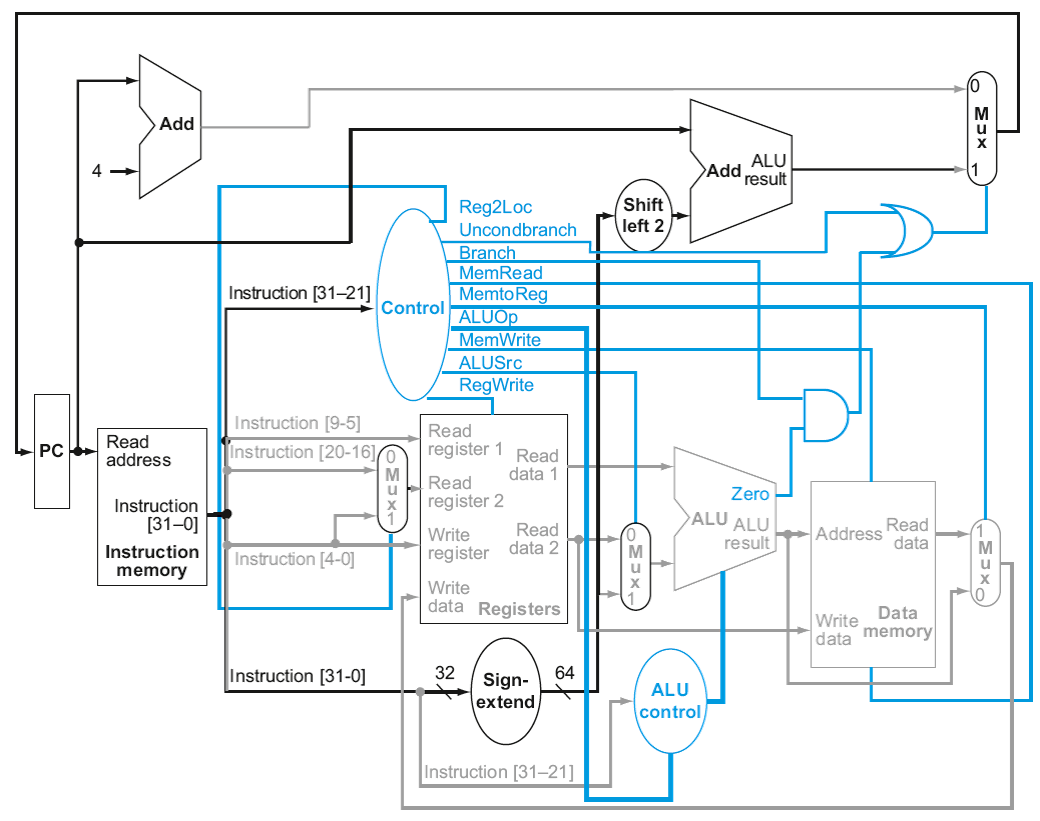
\includegraphics[width=\textwidth]{../images/non_pipelined_datapath.png}
\end{center}
\end{figure}

\section{Your Assignment}

You are to:
\begin{enumerate}
\item Implement the assembly and binary code for the Division C Code shown above.
\item Verify that the divison works correctly.
\item Write up a lab report according to a new format file, LabWriteup.tex.
\end{enumerate} 
%\chapter{Full Datapath}


\section{Datapath}
Now that we have a working single-cycle datapath, we are going to break it apart and start pipelining it.  Make sure to keep a copy of your working single cycle datapath for reference.  To begin the pipelining process, we will first pipeline the iFetch and iDecode stages.

The advantage of pipelining includes the ability to reduce the clock cycle time by doing only one stage at a time.  We have been using a 10ns clock cycle.  Now that we are pipelining, let's start conservative and go down to a 4ns clock cycle.  Please keep it at 4ns for now to maintain consistency across the class.  

This will affect your timing and will require you to update your delays in your datapath.  Ask yourself why you made each delay.  Was it really meant to be relative to the clock cycle time, or was it meant to be a constant number. For instance, if you put in a CYCLE/10 to give a register time to update, do you really want that time to drop from 1ns to 0.4ns?  Has anything about the register update time changed?  The answer is no.  So you need to be strategic with your delays throughout these two stages.  You might also need to modify your delay functions.  The goal for today is to get a series of instructions to execute in pipeline form, where a new instruction is fetched while the previous instruction is being decoded.  You should verify this by examining the Read\_Register values, Read\_Data values, control signal values, etc.  The next step will be buffering nPC and the instruction, but we will focus on that next class.

To test this, use your set of instructions that corresponds to your Expected Results table.

\section{Your Assignment}

You are to:
\begin{enumerate}
\item Comment out Execute, Memory, and WriteBack stages from datapath.v.
\item Pipeline iFetch and iDecode stages and update delays.   
\item Test with your set of instructions from your Expected Results table.
\item Verify that stages are processing the correct instructions at the correct times.
\item There is no lab report today.
\end{enumerate} 
%\chapter{Pipelining without Branching or Forwarding}


\section{Overview}
Now that we can pipeline stages and run them in parallel, we can add the register buffers between each stage and get a simple pipeline working.  This pipeline will not include any data forwarding or branch prediction.  We will handle data hazards by using assembly code with appropriately place nop commands to stall.  For now, we will avoid control hazards by not running any branch instructions.  We will focus on a series of load, arithmetic, and store instructions.

The first step is to create a spreadsheet using the template in this manual directory.  This spreadsheet should detail each input and output of the system.  It will then be filled in with data that needs to be buffered and passed to the next stage.  Please fill out the spreadsheet by doing the following:
\begin{enumerate}
	\item Add all of your inputs and outputs from each module, according to datapath.v.
	\item For each signal, identify the source and destination(s).
	\item For each signal, fill in stages that need the data to be buffered and passed along.  See mem\_to\_reg on template.
	\item For each signal (including the signals to pass along), label the signals with \_if, \_id, \_ie, \_im, or \_iw to indicate what stage that signal is coming from.
	\item Now consider any signals that need to be added due to pipelining, especially signals that go from right to left, such as the register write signals.  Add those to the spreadsheet.
	\item Think through the spreadsheet and determine if you have any holes in your design
\end{enumerate}  

Only after you have completed the spreadsheet as a group (work together on the spreadsheet) and have showed it to me, then you can move on to writing Verilog code.  You will want to update datapath.v to use the names from the spreadsheet.  This will include adding a lot of new signals.  Then you will want to update your modules to account for these new signals.  Try to change as few names as possible within the modules.  You want to use the stage-specific name in datapath.v rather than in the modules, to the extent possible.  Next, you will add procedural statements to assign inputs to register outputs (or in some cases, they will be registers that are internal to the module).  Compile and fix warnings.  Test files (instrData, regData, ramData) have been added to the repository.  Please use these files to test your code.  The assembly for those files is below:

\begin{enumerate}
\item LDUR X9, [X22 , \#0] ;     //load X9 from A[0], X22 = 80, A[0] = 56
\item LDUR X10, [X22 , \#8 ];    //load X10 from A[1], X22 = 80, A[1] = 8
\item LDUR X11, [X22 , \#16];    //load X11 from A[2], X22 = 80, A[2] = 35 
\item LDUR X12, [X22 , \#24];    //load X12 from A[3], X22 = 80, A[3] = 5
\item SUB X9, X9, X10 ; 
\item ADD X11, X11, X12 ; 
\item STUR X9,  [X22 , \#0]
\item STUR X11, [X22 , \#16]
\end{enumerate}
  


\section{Your Assignment}

You are to:
\begin{enumerate}
\item Finish the spreadsheet
\item Implement the spreadsheet in your datapath.v
\item Update your modules to buffer the appropriate values into registers
\item Use the test data files to test the pipeline and correct any issues
\item Submit a lab report using the PipelineLabWriteup format.
\end{enumerate} 
%\chapter{Pipelining with Branching}


\section{Overview}
Once your pipeline is working with the simple set of commands that I provided, it is time to add branching.  

We will put the following restrictions on our efforts to branch:
\begin{enumerate}
	\item Use Branch Not Taken method of prediction
	\item You should move the branch decision hardware to the Decode stage as mentioned in the lecture. 
	\item When a branch is taken, you must zero the control lines and set PCWrite and IF/IDWrite to 0.  You will need to add PCWrite and IF/IDWrite.  Branch hazards must be detected by a new module, the Hazard Detection Unit.
	\item Instructions used for this should be the division problem instructions.  You need to insert nops (all zeros) in the instruction file where necessary.  The only reason to add nops in the instruction file is a data hazard
\end{enumerate}  

\section{Your Assignment}

You are to:
\begin{enumerate}
\item Implement Branch Not Taken Prediction
\item Create an instruction file as described above, based on the division problem instruction file
\item Update your modules to detect and respond to branch hazards
\item Use the instruction to test the pipeline and correct any issues
\item Submit picture(s) of your simulation results.  Also submit a zip file of your repository.
\end{enumerate} 
%\input{buffer}
%\input{control}%and SE
%\input{regfile}
%\chapter{Beginning to Decode}

\section{Instruction Decode}

The next stage in the datapath is the iDecode stage.  The iDecode stage evaluates the binary instructions (an output of the iFetch stage) and determines what needs to be done.  There are many aspects to the iDecode stage, and some get fairly complex.  But today we will begin the process of decoding that instruction by decomposing the instructions into the key parts of R-Type and D-Type instructions:
\begin{enumerate}
	\item Opcode
	\item Address (used only in D-Type instructions)
	\item Rm (used only in R-Type instructions)
	\item Rn
	\item Rd (though the book uses Rt for D-type instructions, we will use Rd for the last operand of D-type instructions)
\end{enumerate}   

To do this, you will create a new module called instr\_parse.  This module will simply read inputs and assign appropriate output values.  These outputs should be assigned on the clock edge with non-blocking procedural assignments.  While this might not seem important now, it will become important later.  The inputs should be a clk signal and a 32-bit instruction.  Outputs are listed for you above.  Although R-type and D-type instructions have different operands, you can treat them the same for now.  For instance, you can still assign an Address field on an R-type instruction, and you can still assign an Rm field on a D-type instruction.  In future labs, we will begin treating the instructions differently and ignore the unnecessary fields.  Notice how because of the commonality of instruction format, Opcode, Rn, and Rd are all universal across these instruction types.  Please remember to use the style specified in the previous lab, where all items are lower case with underscores separating them.  For instance, for Rd, you should use the signal name rd\_num.  Appending num on the end of the name indicates that this is the register number, not the value from the register.

To test this, you will need to create an instr\_parse\_test.v that will feed the module with a clock signal and instructions.  Then you can verify that your instructions are being parsed correctly.

\section{Register File}

Next, we will create the register file.  You will create a new module called regfile (in regfile.v).  The regfile module should retrieve data from the registers on the rising edge of read\_clk as well as write to the registers on the rising edge of write\_clk when the regWrite flag is set.  The regfile should use a verilog reg array.  You do not need to use the register module that you used for your program counter.  Since we don't currently have the ability to do loads and stores (since we don't have data memory yet), the values for the registers should be stored in a datafile, regData.data and read in during the initial block, just like we did with the instr\_mem.v file.  

Inputs to the module should include a signal called read\_clk and a signal called write\_clk as well as all inputs shown on the Register file in Figure~\ref{fig:register_file_cutout}.  The outputs should be the outputs of the Register file in Figure~\ref{fig:register_file_cutout}.  Use names such as read\_register1, read\_data2, etc.

You will need to write a testbench, regfile\_test.v, for this module as well.  It should provide values for each input and verify that the outputs match expected behavior.

\begin{figure}
	\caption{Expected Results}\label{fig:register_file_cutout}
	\begin{center}
		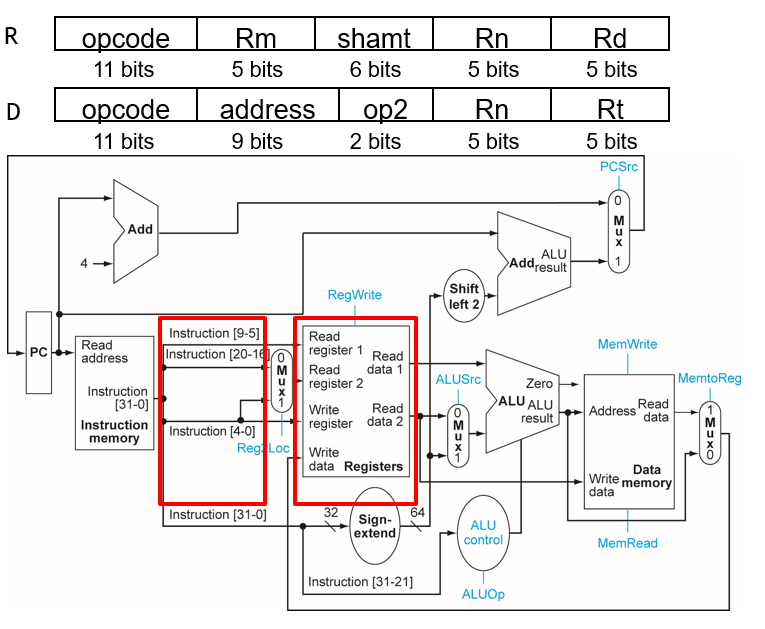
\includegraphics[width=4.75in]{../images/register_file_cutout.png}
	\end{center}
\end{figure} 


\clearpage
\section{Your Assignment}

You are to:
\begin{enumerate}
\item Create an instr\_parse module as described above.
\item Create an instr\_parse test module and verify that the instruction is being parsed properly.
\item Create a regfile module as described above.
\item Create a regfile\_test module and verify that the values are being stored and retrieved from the regfile properly.
\end{enumerate} %and buffer

%midterm
%\chapter{ALU and ALU Control}

\section{ALU}

First we will build the ALU itself.  The ALU has three inputs (two data inputs to act on, and a control input to determine the action perfomed) and two outputs (one data, and a logical flag). In the table shown in the lecture slides, you can see the meaning of the control bits used to determine what the ALU will calculate.  You should use a case statement for the control bits to determine which ALU operation to perform.  For each operation, you do not have to do anything fancy.  You just need to use the math capability that verilog provides to make the calculation.  You should give the the ALU control bits names in the definitions.vh file, and you should use these in your cases.  Also don't forget to make a default case, which is needed to actually wire this up.  Pick something fast for the default, thus usually a logic statement.

One last thing to note is the generation of the zero flag.  There are several ways to handle this, but the easiest way to handle it is below: 
\begin{enumerate}
\item In Verilog (like C), the statement $(a==b)$ is an operation with a boolean output.  You can thus say $x=(a==b);$ to assign $x$ to be the boolean value.  The statement $x=(a==b);$ is realizable as a digital comparator with $a$ and $b$ as inputs and $x$ as the single bit output.
\end{enumerate}

\section{ALU Control}

Now we need to build the controller to use the ALUOp field and the function field to generate the ALU control bits used above.  Consider the table for ALU Op to ALU Control bits in the lecture slides.  The ALU Control module is where you make this translation so that the ALU is told the proper operation to execute.  Use case statements and include a default to handle undefined signals (use fast commands for undefined signals).  Define the ALU operations in definitions.vh file to improve readability - you shouldn't need any numbers.  This should be a simple module with two inputs (ALUOp and function) and one output (control bits).

\section{Your Assignment}

You are to:
\begin{enumerate}
\item I have provided the test bench, ALU\_test.v.
\item Generate an ALU and ALU Control module and verify that you get the results that you expect.
\item Save your simulation results so that they can be included in a lab report.  We will not be submitting a lab report today.
\end{enumerate} %alucontrol, alu
%\chapter{Execute Stage}

\section{Execute}

In the last lab, you created the ALU and ALU Control modules.  Now we will finish the iExecute stage.  The iExecute stage is represented by the red box in Figure ~\ref{fig:execute_stage}.  To finish the iExecute stage, you will need to add the following:
 
\begin{enumerate}
	\item Mux to select the source of the second input into the ALU.  You can reuse your mux that you created in the iFetch stage.
	\item Shifter to left shift the sign extended branch address offset.  You will need to create a new module for this.
	\item Adder to add the branch address offset to the current PC.  You can reuse your adder that you created in the iFetch stage.
\end{enumerate} 

\begin{figure}
	\caption{Execute Stage}\label{fig:execute_stage}
	\begin{center}
		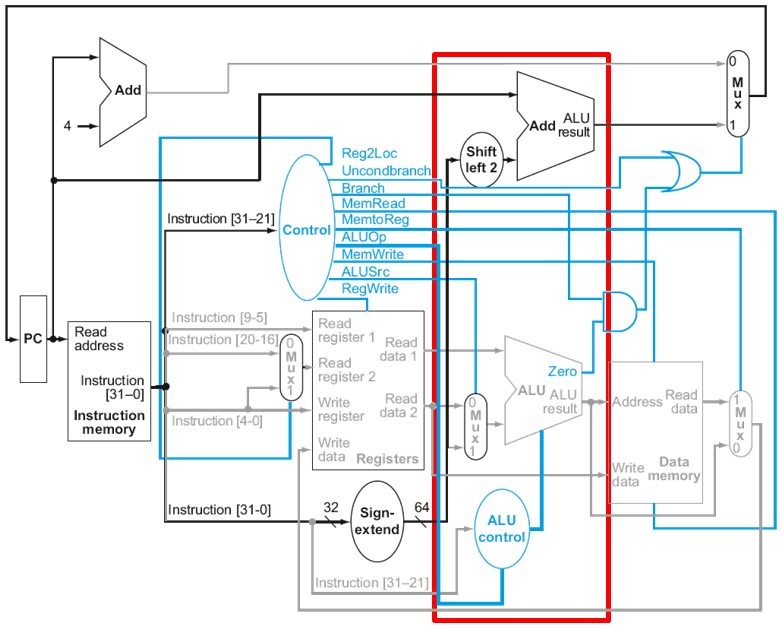
\includegraphics[width=4.75in]{../images/execute_stage.png}
	\end{center}
\end{figure} 

These five modules should be included in a new module called iExecute.  iExecute should consist of everything shown in the red box on Figure ~\ref{fig:execute_stage}. 

\section{Your Assignment}
I have provided a test bench, iExecute\_test.v.  Feel free to modify and improve it as you see fit.

You are to:
\begin{enumerate}
\item Complete the iExecute module and use the iExecute\_test to verify that you get the results that you expect.
\item Do not submit a lab report.  Move straight into Lab 9.
\end{enumerate} %add, mux, buffer
%\input{memory}%and, dmem, buf
%\input{wb}% and pipeline
%\input{coding}%
%\input{performance}%

%\chapter{Bye!}

%\vspace{.1in}

%\begin{center}
%{\Huge{God Bless!}}
%\end{center}

%\vspace{.1in}

%\begin{center}
%{and}
%\end{center}

%\vspace{.1in}

%\begin{center}
%{\Huge{Soli Deo Gloria!}}
%\end{center}


%\appendix
%\input{requirements}
%\input{components}

\end{document} 